\documentclass{article}
\usepackage{graphicx}
\usepackage[margin=1.5cm]{geometry}
\usepackage{amsmath}

\begin{document}
\twocolumn

\title{Wednesday warm-up: Forces I}
\author{Prof. Jordan C. Hanson}

\maketitle

\section{Memory Bank}

\begin{enumerate}
\item $\vec{F}_{\rm net} = 0$ ... Newton's First Law.  If the net force is zero, motion is unchanged.
\item $\vec{F}_{\rm net} = m \vec{a}$ ... Newton's Second Law, relating net force, mass, and acceleration.
\item $\vec{w} = -m g \hat{j}$ ... The weight force on a system with mass $m$.
\end{enumerate}

\section{Chapter 4 - Forces}

\begin{enumerate}
\item Consider Fig. \ref{fig:1}.  If the wagon has a mass of 10 kg, and the child has a mass of 25 kg, what the magnitude and direction of the normal force, $\vec{N}$? \\ \vspace{3cm}
\item Consider Fig. \ref{fig:1}, and neglect the friction force, $\vec{f}$.  If the force of the adult on the wagon and child system is $\vec{F} = 30 \hat{i}$ N, what is the acceleration of the wagon and child? \\ \vspace{3cm}
\item Now take the frictional force into account.  This force comes from the ground pushing on the wheels, which in turn might not have ideal frictionless motion.  The force points to the left, at the bottom of the wheel, giving rise to the clockwise motion of the wheels.  If $\vec{f} = - 5 \hat{i}$ N, what is the acceleration of the wagon and child system? \\ \vspace{3cm}
\end{enumerate}

\begin{figure}
\centering
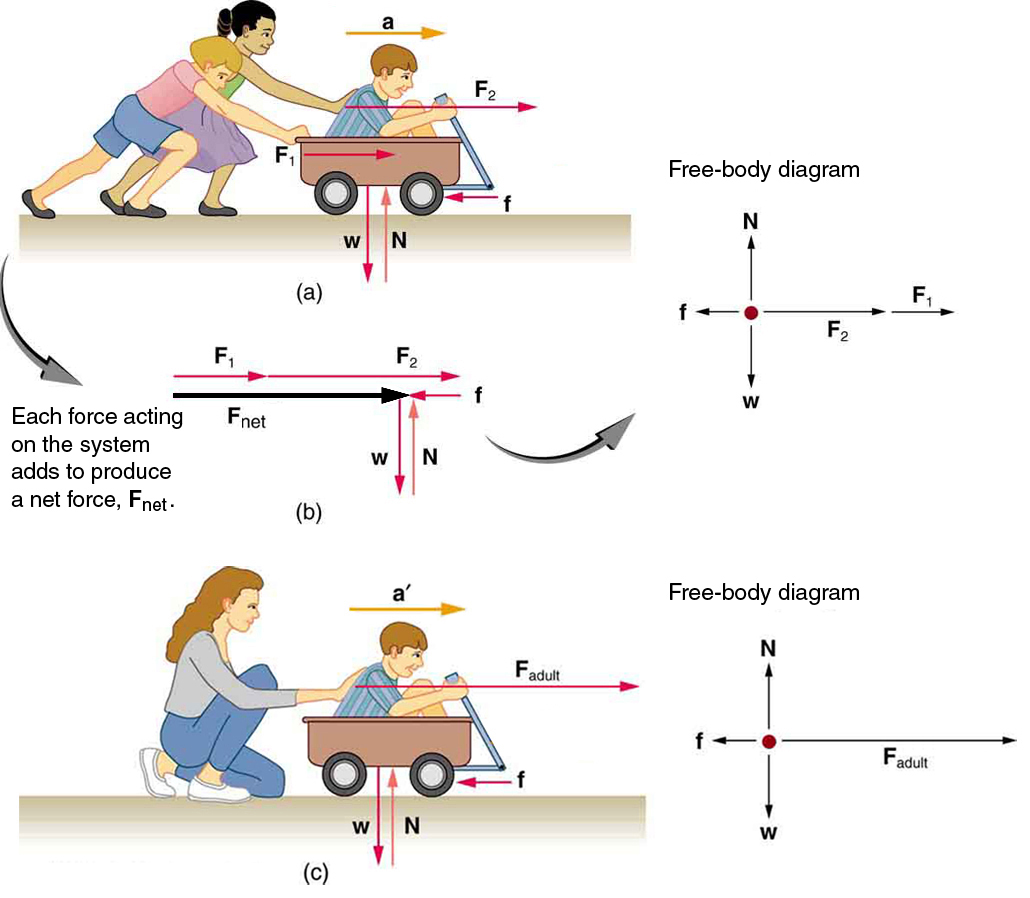
\includegraphics[width=0.5\textwidth,trim=0cm 0cm 0cm 9cm,clip=true]{figures/wagon.jpeg}
\caption{\label{fig:1} A child's wagon, a parent, and a free-body diagram.}
\end{figure}

\end{document}
